\subsection{Динамика манипулятора}\label{part_dynamics}

\subsubsection{Общие замечания}
Введем в рассмотрение барицентрические СК $Ox_{ci}y_{ci}z_{ci}$\lefteqn,\footnote{Системы координат, чьи начала совпадают с центрами масс соответствующих звеньев.} где $i=\overline{1,5}$, показанные на рисунке~\ref{img_mass_frames}.
Заметим, что каждая СК $Ox_{ci}y_{ci}z_{ci}$ сонаправлена с $Ox_iy_iz_i$.

\begin{figure}[h!]
	\centering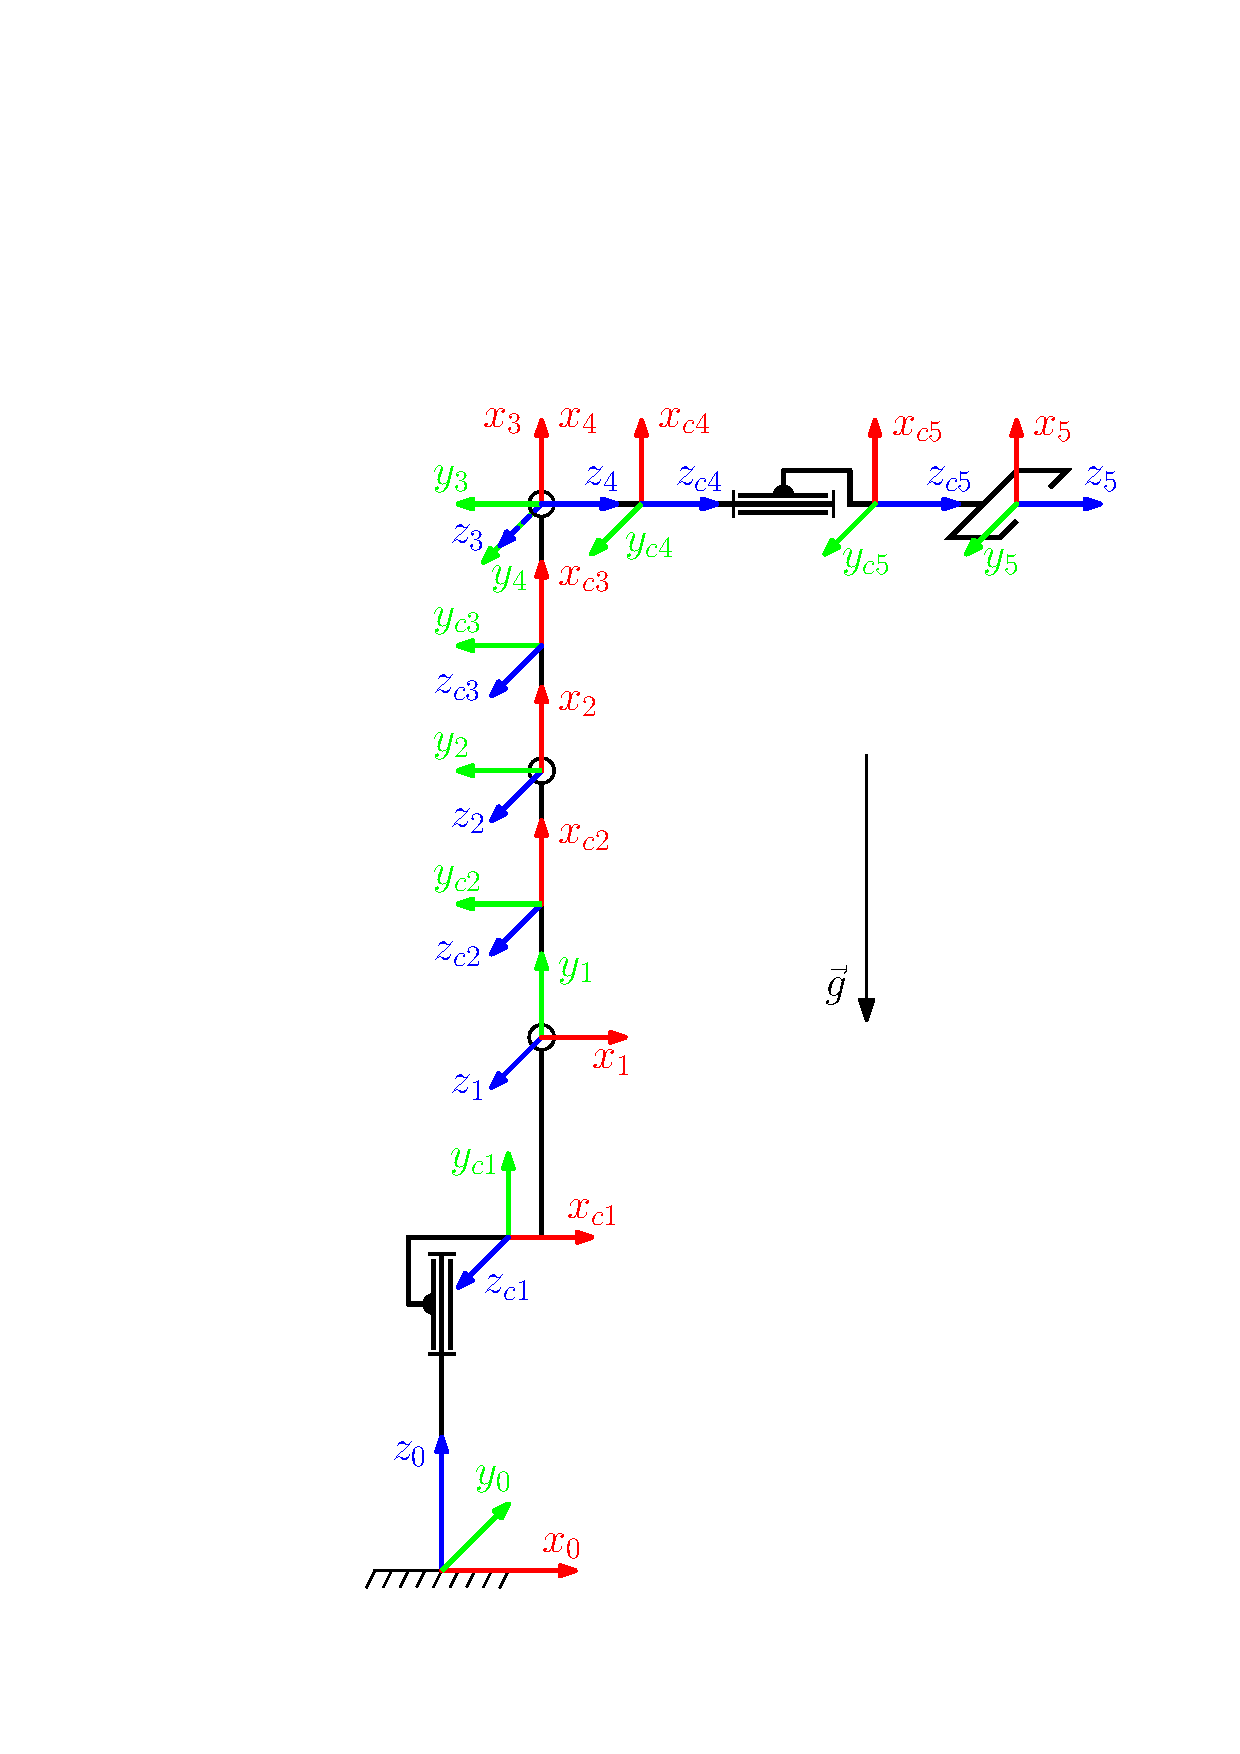
\includegraphics[height=16.5cm]{kinematics_mass_frames.pdf}
	\caption{Положение барицентрических СК и направление вектора $\vec{g}$.}
	\label{img_mass_frames}
\end{figure}

Для описания положения введенных СК воспользуемся следующими векторами:
\begin{equation}
    r^i_{i,\,ci} =
    \begin{bmatrix}
        x_{ci} \\ y_{ci} \\ z_{ci}
    \end{bmatrix}\!\!,\quad i = \overline{1,5},
\end{equation}
где $x_{ci}$, $y_{ci}$ и $z_{ci}$~--- некоторые постоянные величины.

Для компонент тензоров инерции $\mathcal{I}^{ci}_i = const$ введем следующие обозначения:
\begin{equation}
    \mathcal{I}^{ci}_i =
    \begin{bmatrix}
        I_{i,\,xx} & I_{i,\,xy} & I_{i,\,xz} \\
        I_{i,\,xy} & I_{i,\,yy} & I_{i,\,yz} \\
        I_{i,\,xz} & I_{i,\,yz} & I_{i,\,zz}
    \end{bmatrix}\!\!\ldotp
\end{equation}

Заметим, что
\begin{equation}
    g_0 =
    \begin{bmatrix}
        0 \\ 0 \\ -g
    \end{bmatrix}\!\!,
\end{equation}
где $g=9.82\text{ м}/\text{с}^2$.

В~заключении раздела приведем формулы для расчета величин, которые потребуются в дальнейшем (везде $i = \overline{1,5}$):
\begin{itemize}
    \item для расчета $r^0_{0,\,i}$ и ${}^{0}R_i$ (см.~Приложение~\ref{app_ht_matrices}):
        \begin{equation}
            {}^0A_i = {}^0A_1 \cdot {}^1A_2 \cdot \ldots \cdot {}^{i-1}A_i;
        \end{equation}
    \item для расчета $r^0_{0,\,ci}$:
        \begin{equation}
            \begin{bmatrix}
                r^0_{0,\,ci} \\ 1
            \end{bmatrix}
            = {}^0A_i
            \begin{bmatrix}
            r^i_{i,\,ci} \\ 1
            \end{bmatrix}\!\!;
        \end{equation}
    \item для расчета $r^i_{i-1,\,i}$:
        \begin{gather}
            {}^{i-1}A_i \quad \Rightarrow \quad {}^{i-1}R_i,\: r^{i-1}_{i-1,\,i},
            \\
            r^i_{i-1,\,i} = {}^{i-1}R_i^{-1} \!\cdot r^{i-1}_{i-1,\,i};
        \end{gather}
    \item для расчета $z^0_i$:
        \begin{equation}
            z^0_i = {}^{0}R_i \cdot z^i_i = {}^{0}R_i \cdot
            \begin{bmatrix}
                0 \\ 0 \\ 1
            \end{bmatrix}\!\!\ldotp
        \end{equation}
\end{itemize}

\subsubsection{Получение уравнений движения методом Эйлера-Лагранжа}
Потенциальная энергия манипулятора
\begin{equation}
    U = -g_0^T \cdot \sum_{i = 1}^5 m_ir^0_{0,\,ci} =
\end{equation}

Якобианы, устанавливающие в соответствии с формулой
\begin{equation}
    v^0_{ci} = J_{vi}\dot{q}, \quad i = \overline{1,5}
\end{equation}
связь между линейными скоростями центров масс звеньев и вектором~$\dot{q}$:
\begin{gather}
    J_{v1} =
    \begin{bmatrix}
        z^0_0 \times \left( r^0_{0,\,c1} - r^0_{0,\,0}\right) & \nv & \nv & \nv & \nv
    \end{bmatrix}\!\!,
    \\
    J_{v2} =
    \begin{bmatrix}
        z^0_0 \times \left( r^0_{0,\,c2} - r^0_{0,\,0}\right) & z^0_1 \times \left( r^0_{0,\,c2} - r^0_{0,\,1}\right) & \nv & \nv & \nv
    \end{bmatrix}\!\!,
    \\
    J_{v3} =
    \begin{bmatrix}
        z^0_0 \times \left( r^0_{0,\,c3} - r^0_{0,\,0}\right) & z^0_1 \times \left( r^0_{0,\,c3} - r^0_{0,\,1}\right) &
        z^0_2 \times \left( r^0_{0,\,c3} - r^0_{0,\,2}\right) & \nv & \nv
    \end{bmatrix}\!\!,
    \\
    J_{v4} =
    \begin{bmatrix}
        z^0_0 \times \left( r^0_{0,\,c4} - r^0_{0,\,0}\right) \\
        z^0_1 \times \left( r^0_{0,\,c4} - r^0_{0,\,1}\right) \\
        z^0_2 \times \left( r^0_{0,\,c4} - r^0_{0,\,2}\right) \\
        z^0_3 \times \left( r^0_{0,\,c4} - r^0_{0,\,3}\right) \\
        \nv
    \end{bmatrix}^T\!\!\!\!\!,
    \qquad
    J_{v5} =
    \begin{bmatrix}
        z^0_0 \times \left( r^0_{0,\,c5} - r^0_{0,\,0}\right) \\
        z^0_1 \times \left( r^0_{0,\,c5} - r^0_{0,\,1}\right) \\
        z^0_2 \times \left( r^0_{0,\,c5} - r^0_{0,\,2}\right) \\
        z^0_3 \times \left( r^0_{0,\,c5} - r^0_{0,\,3}\right) \\
        z^0_4 \times \left( r^0_{0,\,c5} - r^0_{0,\,4}\right)
    \end{bmatrix}^T\!\!\!\!\!,
\end{gather}
где $\nv = [0\;0\;0]^T$~--- нулевой вектор.

Якобианы, устанавливающие в соответствии с формулой
\begin{equation}
    \omega^0_{ci} = J_{\omega i}\dot{q}, \quad i = \overline{1,5}
\end{equation}
связь между угловыми скоростями звеньев и вектором~$\dot{q}$:
\begin{gather}
    J_{\omega 1} =
    \begin{bmatrix}
        z^0_0 & \nv & \nv & \nv & \nv
    \end{bmatrix}\!\!,
    \qquad
    J_{\omega 2} =
    \begin{bmatrix}
        z^0_0 & z^0_1 & \nv & \nv & \nv
    \end{bmatrix}\!\!,
    \\
    J_{\omega 3} =
    \begin{bmatrix}
         z^0_0 & z^0_1 & z^0_2 & \nv & \nv
    \end{bmatrix}\!\!,
    \qquad
    J_{\omega 4} =
    \begin{bmatrix}
        z^0_0 & z^0_1 & z^0_2 & z^0_3 & \nv
    \end{bmatrix}\!\!,
    \\
    J_{\omega 5} =
    \begin{bmatrix}
        z^0_0 & z^0_1 & z^0_2 & z^0_3 & z^0_4
    \end{bmatrix}\!\!\ldotp
\end{gather}

Кинетическая энергия манипулятора:
\begin{equation}
    K = \frac{1}{2}\, \dot{q}^T \left( \sum_{i=1}^5 \left( m_i J_{vi}^T J_{vi} + J_{\omega i}^T \, {}^0\!R_i \, \mathcal{I}^{ci}_i \, {}^0\!R_i^T J_{\omega i} \right) \right) \dot{q} =
\end{equation}

Функция Лагранжа
\begin{equation}
    L = K - U\ldotp
\end{equation}

Уравнения движения робота:
\begin{equation}
    \frac{d}{dt}\frac{\partial L}{\partial\dot{q_i}} - \frac{\partial L}{\partial q_i} = \tau_i, \quad i = \overline{1,5} \qquad \Rightarrow
\end{equation}
\begin{equation}
    \Rightarrow \quad
	\left\{
	\begin{aligned}
		\!& = \tau_1\\
		\!& = \tau_2\\
		\!& = \tau_3\\
		\!& = \tau_4\\
		\!& = \tau_5
	\end{aligned}
	\right.
\end{equation}
\newpage
